\hspace{24pt}
In this section, first we introduce dataset and some tools, then we will explain the steps of our experiment, analyze the experimental results in three different simulation scenarios, and finally discuss results using the VCF file from dbSNP divided it into SNPs and indels.

\section{Dataset}
EAGLE needs three main input files: the reference genome (FASTA), read data (FASTQ), and a variant file (VCF). 

First, the reference genome sequencing data we used is Genome Reference Consortium Human Build 37 patch release 13 (GRCh37.p13) version from NCBI website.  It includes autosomal chromosomes 1 to 22, X and Y chromosome of primary assembly and some extra sequences.

Second, the read sequencing data is real sequencing data from NA12878 which is a cell line of an individual female from a CEPH pedigree that is Utah residents with Northern and Western European ancestry, using an exome sequencing dataset (Garvan HG001) by sequencer HiSeq2500 from Genome-In-A-Bottle (GIAB).

Third, we will use VCF files from the Single Nucleotide Polymorphism Database (dbSNP). dbSNP is a public domain archive for a wide collection of simple genetic polymorphisms. The polymorphism set includes single bases nucleotide substitutions (also called single nucleotide polymorphisms or SNPs), and small-scale base deletions or insertions (indels).

Finally, we will also use a simulated VCF file, the variant file is generated by our simulation, we provide more details below.

\section{Simulation workflow}
In order to carefully evaluate the effect of our modifications to EAGLE and verify whether our method can reduce the influence of reference bias, we use simulation methods to conduct experiments.  We modify the GRCh37 reference genome sequence to simulate the occurrence of differences between a reference genome and an individual genome (Figure~\ref{simulate_variants}), and record the result of our modification to generate a VCF file.  We refer to variants simulated in this way as ``planted variants'' and the resulting modified reference as the ``doctored reference''.  An advantage of this approach is real read data can be used.  A disadvantage is that only homozygous variants can be simulated.

\begin{figure}[ht]
\vspace{1em}
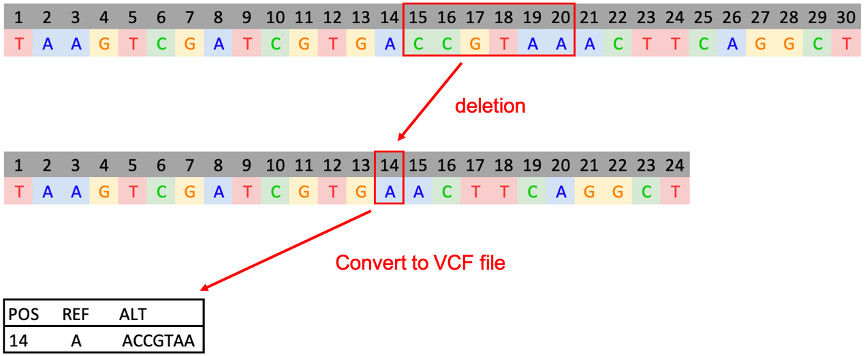
\includegraphics[width=1\columnwidth]{body/image/simulate_variants.png}
\caption[Simulate variants]{Simulate variants.}
\label{simulate_variants}
\end{figure}

Then we will use BWA, following the traditional approach, and do the read mapping alignment again, to obtained a doctored reference pile-up.  Use the re-alignment step to simulate the occurrence of reference bias, because we modified the reference, when re-aligning, the pileup at the original position will have some reads affected by the change we made to the reference, and these affected reads will be misaligned or perhaps mapped elsewhere. After generating the files needed by EAGLE, we can start our experiment.  The entire experiment process is outlined in Figure~\ref{simulation_workflow}.

\begin{figure}[ht]
\vspace{1em}
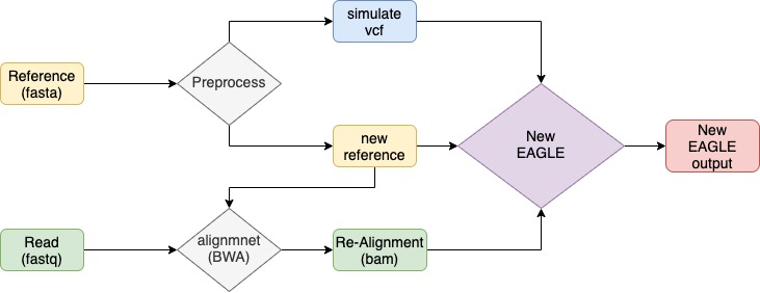
\includegraphics[width=1\columnwidth]{body/image/simulation_workflow.png}
\caption[Simulation workflow]{Simulation workflow.}
\label{simulation_workflow}
\end{figure}

In order to analyze the affect of read depth on our results, we used SAMtools to check the original reference pile-up read depth, and divide genome positions into three categories of pileup read depth: 5--20x, 20--40x and \textgreater40x (Table~\ref{tab:simulate-amount}).

\begin{table}[ht]
\center
\caption[total simulate indels amount]{total simulate indels amount}
\vspace{-1em}
\begin{tabular}{|l|c|c|c|}
\hline
\rowcolor{lightgray}
\textbf{Pile-up Read Depth}&    \textbf{5x -- 20x} &    \textbf{20x -- 40x} &    \textbf{$>$ 40x}\\
\hline
\cellcolor{lightgray}\textbf{Indel length} &   1 -- 50&     1 -- 50&     1 -- 50\\
\hline
\cellcolor{lightgray}\textbf{Amount} &   20 for each&    20 for each&     20 for each\\
\hline
\cellcolor{lightgray}\textbf{Total variants} &   1000&     1000&     1000\\
\hline
\end{tabular}
\label{tab:simulate-amount}
\end{table}


For each read depth category, and each length $l$ from 1 to 50, we randomly selected 20 positions and deleted a string of $l$ base pairs from the standard reference genome to obtain a doctored reference genome.  We do this to simulate insertion variants, as the read data (which is real and presumably matches the standard reference genome in most positions) should contain the sequences we deleted from the reference.  While examining the affect of indel length on our results we will discuss the results after re-alignment in two situations, one is that after re-alignment to the doctored reference, BWA still aligns some reads to the planted variant position, and the other is that after re-alignment, no read can be aligned to that position.

In the first case, the original EAGLE is still able to evaluate the variants, so the focus of our discussion will be the changes in EAGLE evaluation after the introduction of our method. For the second case, we will focus on the new results calculated by EAGLE.

\begin{samepage}
\noindent
Our evaluation is based on the log odds ratio output of EAGLE of each variant $v$:
%%
\begin{equation*}
\log \frac{\text{P}[\text{Alt} | v]}{\text{P}[\text{Ref} | v]}
\end{equation*}
\end{samepage}


\section{Case 1: Low read depth}
The first two rows of Table \ref{tab:low-variants} show how often the EAGLE likelihood ratio changes after adding any new reads from our read index into consideration.
We can see that in the case of low read depth, since only a small number of reads are mappable at all (even against the original reference sequence), once there is a reference bias (simulated by mapping against the doctored reference), EAGLE's evaluation can easily be severely affected.  As expected, you can also see that the longer the length of indels, the more serious the impact.

\begin{table}[ht]
\center
\caption[low read depth variants]{low read depth variants}
\vspace{-1em}
\begin{tabular}{|l|l|l|l|l|l|l|l|l|l|l|r|}
\hline
\textbf{Indel Length} & 
\multicolumn{2}{c|}{\textbf{1--10}}  & \multicolumn{2}{c|}{\textbf{11--20}}  & \multicolumn{2}{c|}{\textbf{21--30}}  &
\multicolumn{2}{c|}{\textbf{31--40}}  & \multicolumn{2}{c|}{\textbf{41--50}}   & 
\textbf{Total}\\\hline
\rowcolor{lightgray}
\textbf{Unchanged}  & 
47 & 42\%       &
38 & 41.8\%     &
30 & 29.1\%    &
10 & 19.2\%     &
0 & 0\%          &
125\\ \hline
\textbf{Changed} & 
65 & 58\%       &
53 & 58.2\%     & 
73 & 70.9\%    & 
42 & 80.8\%     &
5 & 100\%        &
238\\ \hline
\rowcolor{lightgray}    
\textbf{New}  & 
\multicolumn{2}{c|}{88}      &
\multicolumn{2}{c|}{109}     &
\multicolumn{2}{c|}{97}      &
\multicolumn{2}{c|}{148}    &
\multicolumn{2}{c|}{195}       & 
637\\ \hline
\end{tabular}
\label{tab:low-variants}
\end{table}

Next, let’s take a look at the changes after adding our read-index based method.  As shown in table~\ref{tab:low-variants-change}, EAGLE predicts that the position does not contain variants when only using the doctored reference pile-up; but in most cases (19 out of 23), when we find some reads matching the variants, we can help EAGLE judge whether the position contains variants. 

\begin{table}[ht]
\center
\caption{Number of planted variants missed at low read depth}
\begin{tabular}{|l|c|c|c|c|c|r|}
\hline
\diagbox[dir=NW,width=12em]{$\frac{\mathbf{P}[\text{Alt}]}{\mathbf{P}[\text{REF}]} < 1$}{\textbf{Indel length}} &
\textbf{1--10} & \textbf{11--20} & \textbf{21--30} & \textbf{31--40} & \textbf{41--50} & \textbf{Total}\\
\hline
\rowcolor{lightgray}
\textbf{Before} &  7&     2&     3&    4&   3&   19 \\
\hline
\textbf{After} &   2&     1&     0&    1&   0&    4 \\
\hline
\end{tabular}
\label{tab:low-variants-change}
\end{table}

We checked the cases that changed after we found the read, and we found that most of the examples were as we predicted, and we were able to find reads that were misaligned due to reference bias. Figure~\ref{low_new_ALTread} is one of the cases.

\newcommand*{\ExplainRedBracket}{The original reference genome is displayed at top, with a red bracket indicating the variant sequence deleted from our doctored reference}


\begin{figure}[H]
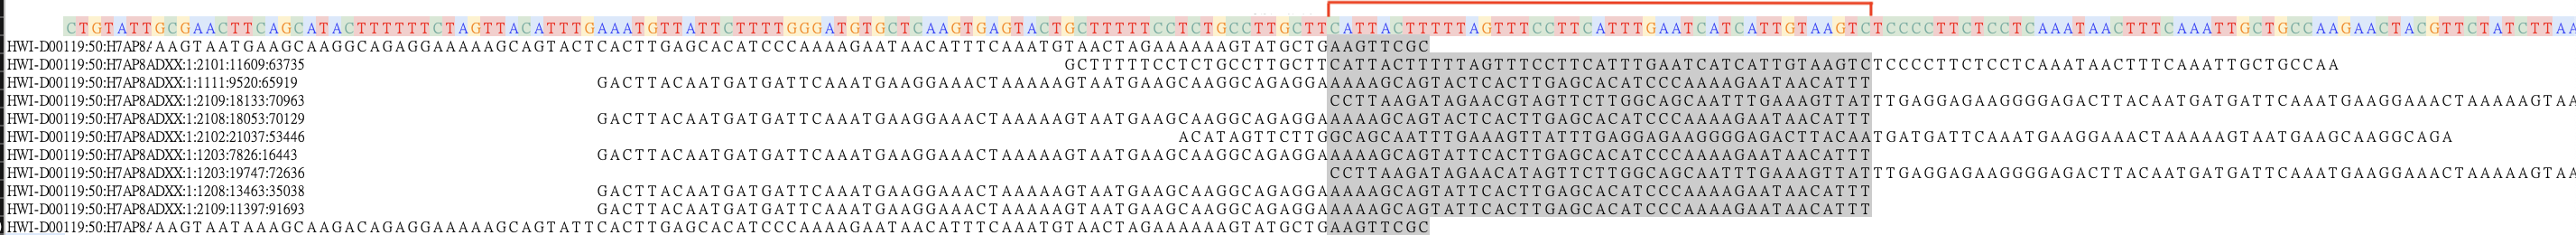
\includegraphics[width=1\columnwidth]{body/image/low_new_ALTread.png}
\caption[New reads in a region with low pile-up read depth]
{Example of new reads supporting a variant in a region with low pile-up read depth.
\ExplainRedBracket.
}
\label{low_new_ALTread}
\end{figure}

Similarly, especially in repetitive genome regions, there are some new reads which are also similar to the reference sequence (Figure \ref{low_new_REFread}).

\begin{figure}[H]
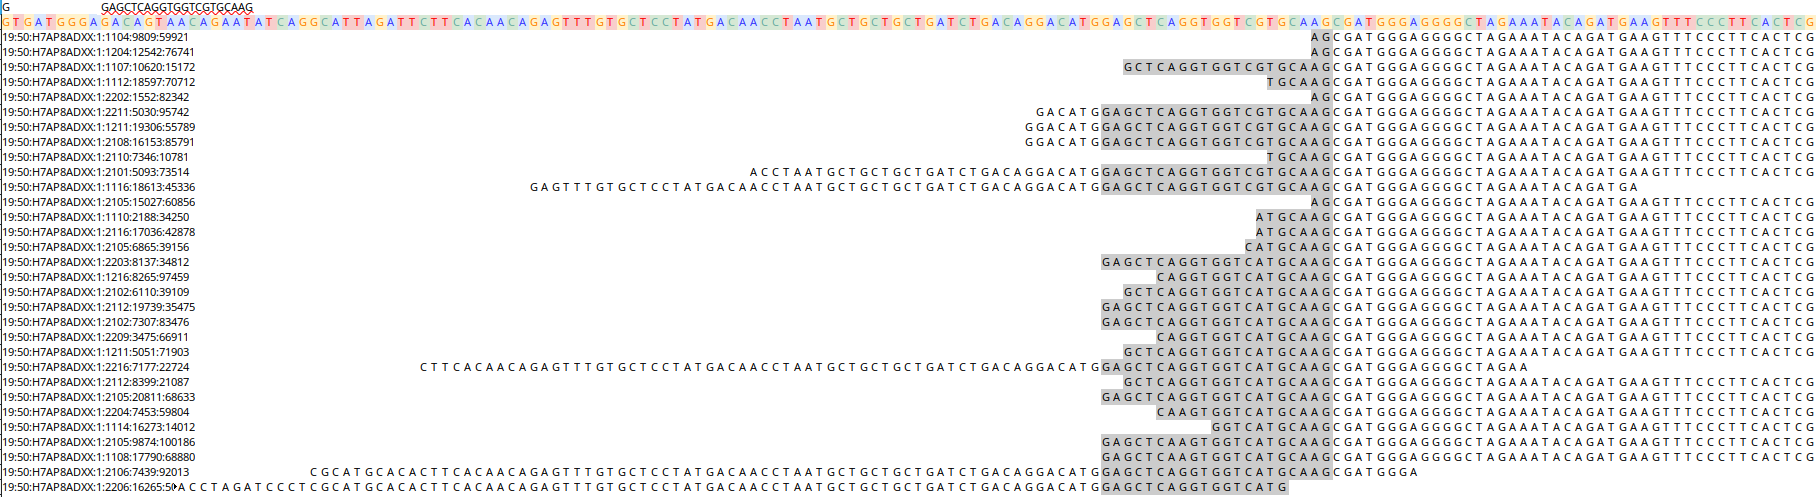
\includegraphics[width=1\columnwidth]{body/image/low_new_REFread.png}
\caption[New reads are similar to the reference with low pile-up read depth]
{Example where new reads found are also similar to the reference sequence with low pile-up read depth.
\ExplainRedBracket.
Note the repetitive nature of the surrounding genome sequence.}
\label{low_new_REFread}
\end{figure}

Next, we can look at the comparison of EAGLE log odds ratio.
\begin{equation*}
\text{log odds ratio change} = \text{log odds(after)} - \text{log odds(before)}
\end{equation*}
to represent the effect of our new method on EAGLE candidate variant evaluation.

\begin{figure}[H]
\centering
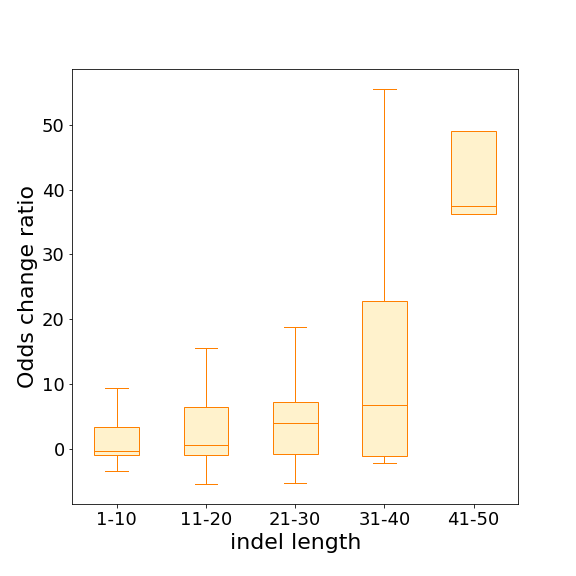
\includegraphics[width=0.6\columnwidth]{body/image/low_odds_change.png}
\caption[low pile-up read depth odds change ratio]
{The vertical axis shows the change in EAGLE log odds ratio of variant to reference for indel variants, grouped by length (horizontal axis).  Change here means the difference in the log odds ratio when using the read index versus only using the pile-up.  Plotted for variants from low pile-up read depth regions.}
\label{low_odds_change}
\end{figure}

In the case of low pile-up read depth, first of all, we can observe that after we add reads, the confidence value of most of the variants increases because we find more reads that contain the variant sequence (Figure \ref{low_odds_change}), and regardless of the length of the indel, their distribution of logs odds ratio change is mostly above zero.
This may mean that even in the case of low pile-up read depth, our method is very helpful for most mutation points, especially for indels with a length of 40 or more, where the increase is particularly obvious.

Finally, we look at the last row of Table \ref{tab:low-variants-change}, we can see these positions are affected by the reference bias, so that no read can be mapped to these positions to form a pileup. Our method is obviously very helpful. For the remaining variants in the 1,000 variants, we can find those reads that are affected by reference bias and are lost, thereby helping EAGLE evaluate the possibility of these mutations.

\begin{figure}[H]
\centering
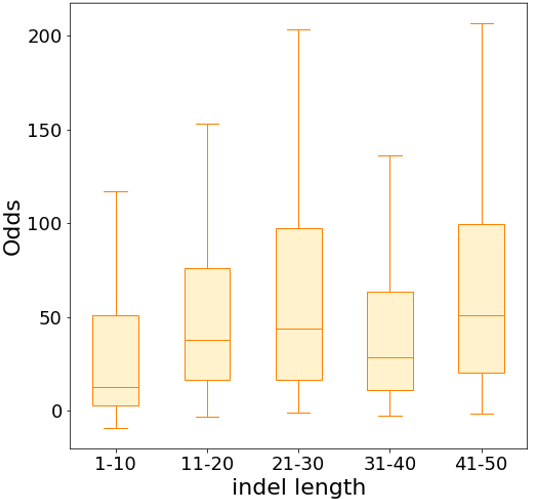
\includegraphics[width=0.6\columnwidth]{body/image/low_new_odds.png}
\caption[no reads with variants from low pile-up depth odds ratio]{The vertical axis shows the EAGLE log odds ratio of variant to reference for indel variants, grouped by length (horizontal axis).  Plotted for variants occurring in regions with no reads from low pile-up depth.}
\label{low_new_odds}
\end{figure}

Then see the odds calculated by EAGLE after we find the read (Figure \ref{low_new_odds}), we can see the odds calculated by EAGLE. For most of the variants, EAGLE gives the conclusion the variant occurs at this position, which is also in line with our expected results.


\section{Case 2: Medium pile-up read depth}
\begin{center}
\begin{table}[h]
    \centering
    \caption[medium pile-up read depth variants]{medium pile-up read depth variants}
    \vspace{-0.5cm}
    \begin{tabular}{|l|l|l|l|l|l|l|l|l|l|l|r|}
    \hline
    \textbf{Indel Length} & 
    \multicolumn{2}{c|}{\textbf{1--10}}  & \multicolumn{2}{c|}{\textbf{11--20}}  & \multicolumn{2}{c|}{\textbf{21--30}}  &
    \multicolumn{2}{c|}{\textbf{31--40}}  & \multicolumn{2}{c|}{\textbf{41--50}}   & 
    \textbf{Total}\\\hline
    \rowcolor{lightgray}
    \textbf{Unchanged}  & 
    36 & 28.3\%       &
    21 & 13.4\%     &
    25 & 15.8\%    &
    33 & 20.4\%     &
    22 & 17.1\%          &
    137\\ \hline
    \textbf{Changed} & 
    91 & 71.7\%       &
    136 & 86.6\%     & 
    133 & 84.2\%    & 
    129 & 79.6\%     &
    107 & 82.9\%        &
    596\\ \hline
    \rowcolor{lightgray}    
    \textbf{New}  & 
    \multicolumn{2}{c|}{72}      &
    \multicolumn{2}{c|}{41}     &
    \multicolumn{2}{c|}{42}      &
    \multicolumn{2}{c|}{38}    &
    \multicolumn{2}{c|}{71}       & 
    264\\ \hline
    \end{tabular}
    \label{tab:mid-variants}
\end{table}
\end{center}

First of all, we can see that in this case, Table~\ref{tab:mid-variants}, because of the increase in the original pile-up read depth, the variants which cannot be called due to reference bias are significantly reduced, and the number of reads that we can overlap with the variant position also increased. For the same reason, more misaligned reads are affected by reference bias.

\begin{table}[ht]
    \centering
    \caption[Changes in the number of variants with medium pile-up read depth]{Changes in the number of variants with medium pile-up read depth}
    \vspace{-0.5cm}
    \begin{tabular}{|l|c|c|c|c|c|r|}
    \hline
    \diagbox[dir=NW,width=12em]{$\frac{\mathbf{P}[\text{Alt}]}{\mathbf{P}[\text{REF}]} < 1$}{\textbf{Indel length}} &
    \textbf{1--10} &     \textbf{11--20} &    \textbf{21--30} &    \textbf{31--40} &    \textbf{41--50} &    \textbf{Total}\\
    \hline
    \rowcolor{lightgray}
    \textbf{Before} &   10&     11&     9&    6&   5&    41 \\
    \hline
    \textbf{After} &   1&     1&     0&    1&   0&    3 \\
    \hline
    \end{tabular}
    \label{tab:mid-variants-change}
\end{table}

With the same increase in pile-up read depth, In EAGLE’s initial judgment, the computed likelihood that position does not contain the variant has also increased, because more misalignments have occurred. And just for this reason, the more reads that we can find to help EAGLE. Therefore, we can see that after we find the misaligned reads, the affect on variant evaluation has also increased, nearly 91\% of variants in Table \ref{tab:mid-variants-change} have been changed to the correct situation. Figures~\ref{mid_new_ALTread} and \ref{mid_new_REFread} show some examples.


\begin{figure}[H]
\centering
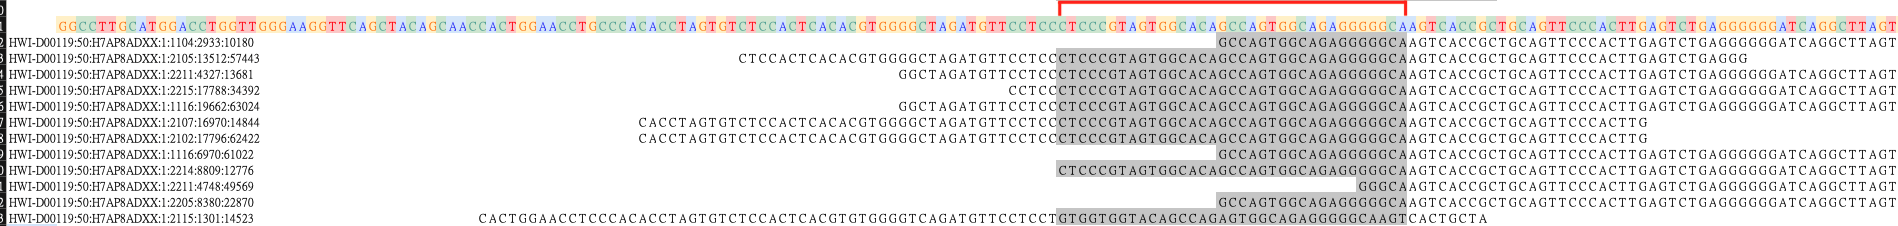
\includegraphics[width=1\columnwidth]{body/image/mid_new_ALTread.png}
\caption[New reads in a region with medium pile-up read depth]
{Example of new reads supporting a variant in a region with medium pile-up read depth.
\ExplainRedBracket.}
\label{mid_new_ALTread}
\end{figure}

\begin{figure}[H]
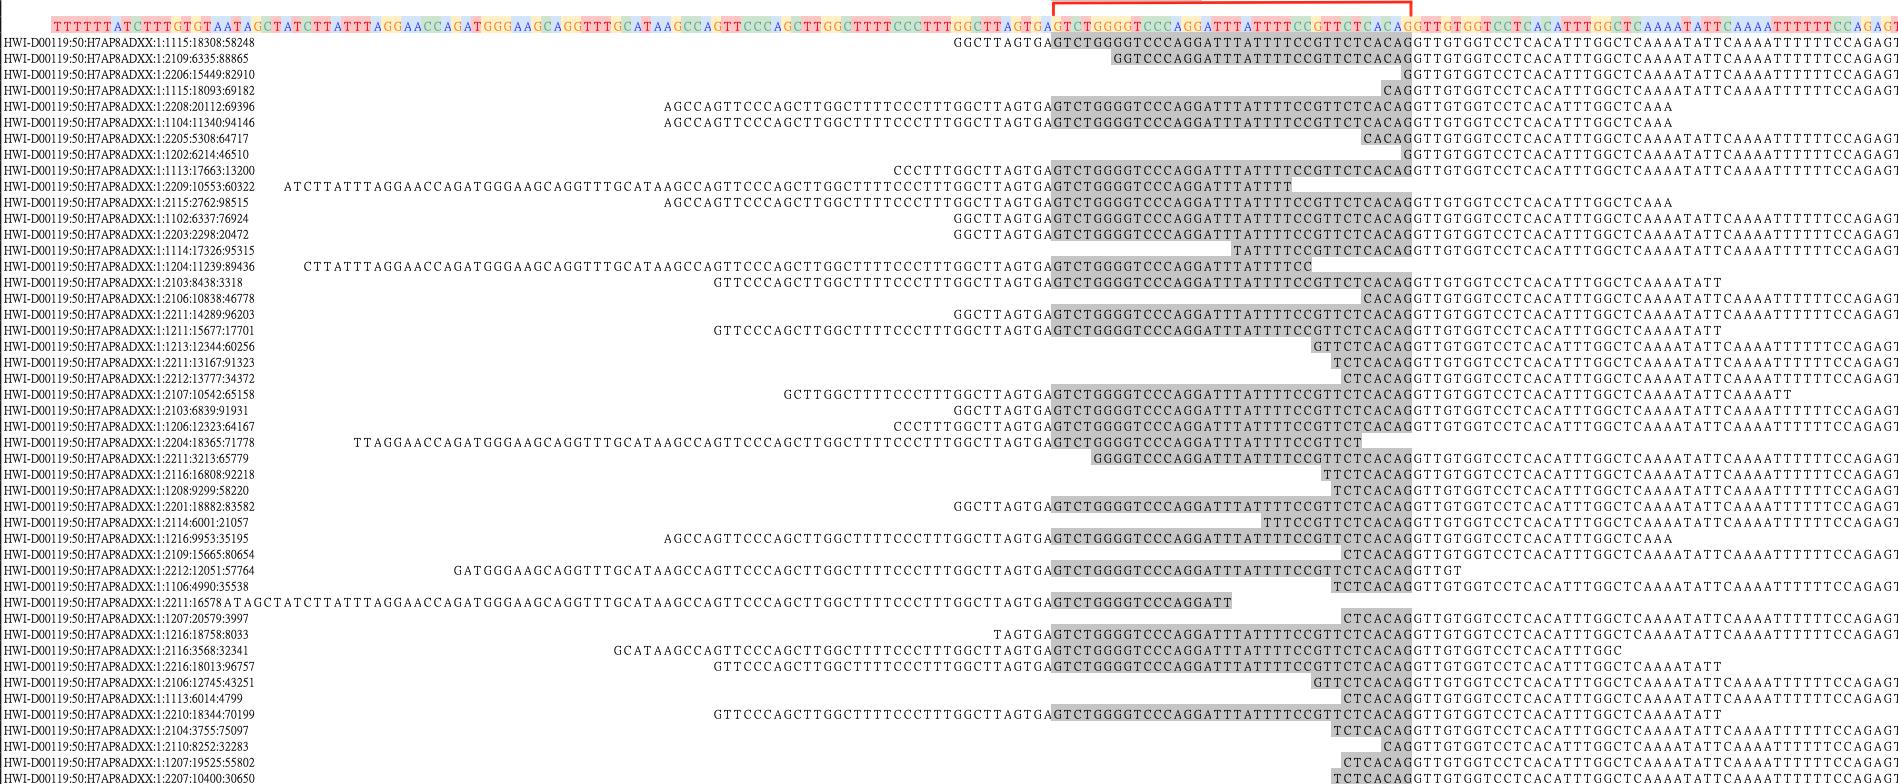
\includegraphics[width=1\columnwidth]{body/image/mid_new_REFread.png}
\caption[New reads are similar to the reference with medium pile-up read depth]
{Example where new reads found are also similar to the reference sequence with medium pile-up read depth.
\ExplainRedBracket.
Note the repetitive nature of the surrounding genome sequence.}
\label{mid_new_REFread}
\end{figure}

We can find that in bad cases, although we found reads similar to hypothetical variant sequences, we did not improve the score of EAGLE on variants. In these few examples, we found that their mutated sequences happened to be repeated sequences. Therefore, the similarity between it and the reference sequence is also very high (Figure \ref{mid_pileup_REFread}).


\begin{figure}[H]
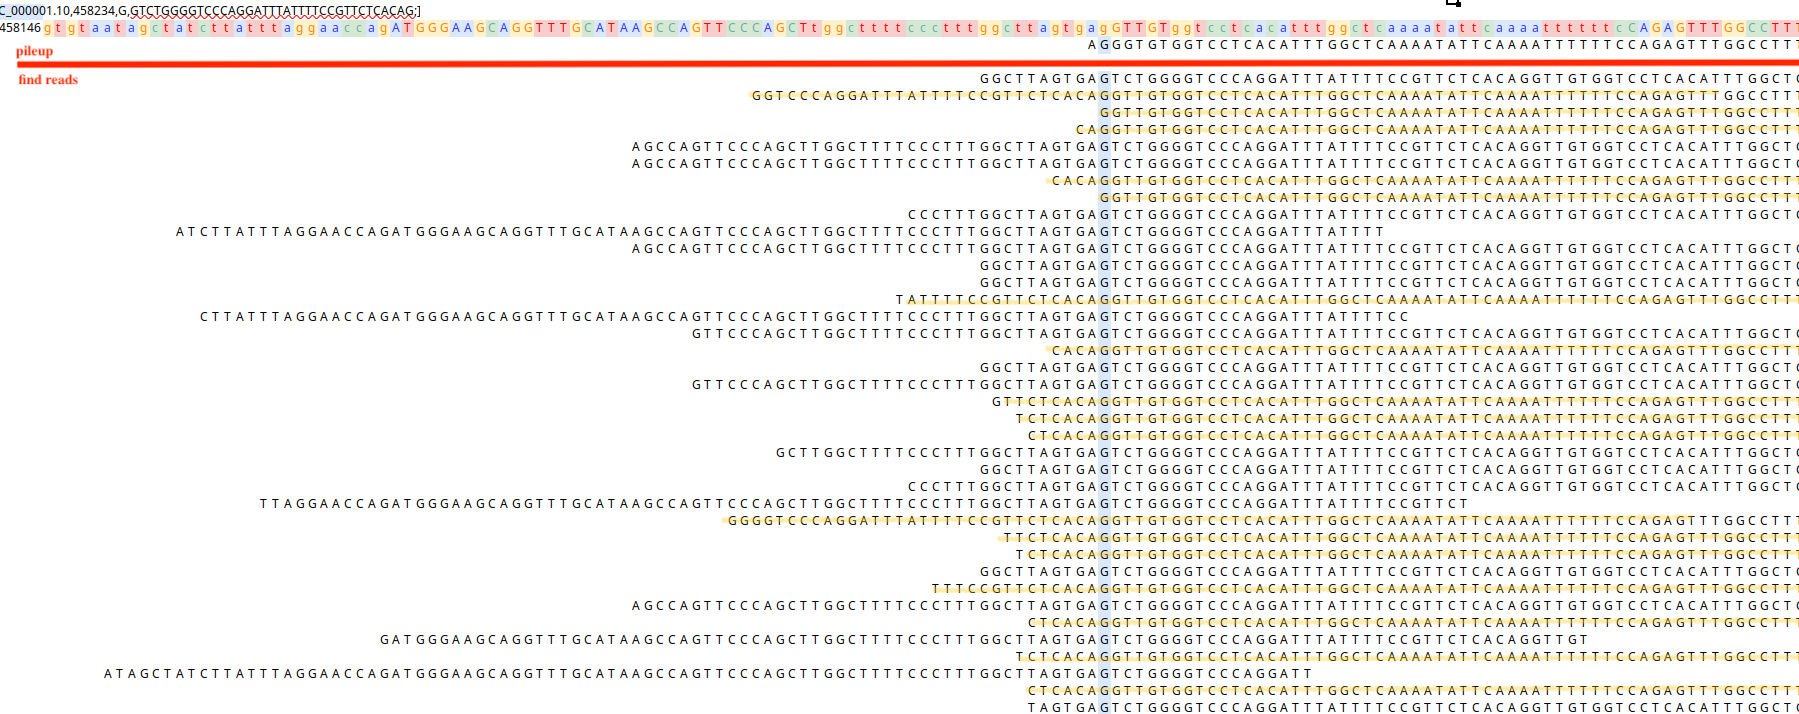
\includegraphics[width=1\columnwidth]{body/image/mid_pileup_REFread.png}
\caption[pileup with Figure~\ref{mid_new_REFread}]
{The pile-up of reads aligned to the doctored genome for the variant from Figure~\ref{mid_new_REFread}.
At top, the doctored reference genome is shown with an arrow indicating where the simulated variant sequence was deleted from the original reference.}
\label{mid_pileup_REFread}
\end{figure}


\begin{figure}[H]
\centering
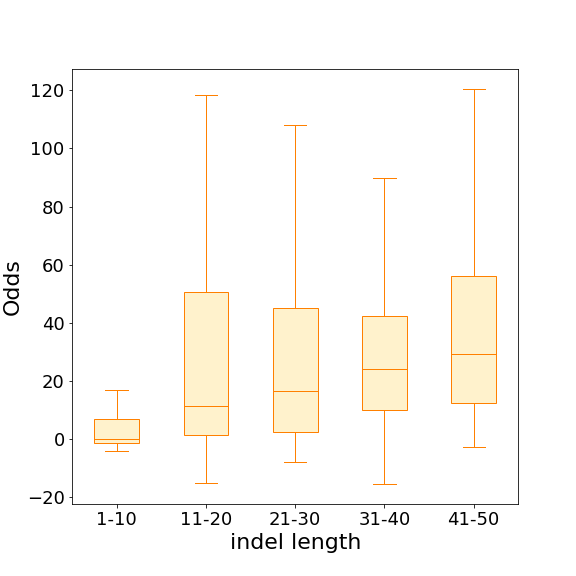
\includegraphics[width=0.6\columnwidth]{body/image/mid_odds_change.png}
\caption[medium pile-up read depth odds change ratio]{The vertical axis shows the change in EAGLE log odds ratio of variant to reference for indel variants, grouped by length (horizontal axis).  Change here meaning the difference in the log odds ratio when when using the read index versus only using the pile-up.  Plotted for variants from medium pile-up read depth regions.}
\label{mid_odds_change}
\end{figure}

Next, we can look at the comparison of EAGLE odds change for medium pile-up read depth (Figure \ref{mid_odds_change}). Basically, the change is similar to the situation of low pile-up read depth. We can also see larger change for longer indels. The difference is that we also have a good performance in the shorter indel. And the average change is better than that of low pile-up read depth. This result is quite reasonable, because we find more reads that match the variant, which can help EAGLE give these mutations greater confidence.
We can also see that indels with a length of 10 or more on our box plot have Q3 greater than 0, which means that most of our reads can help us eliminate the influence of reference bias.

\begin{figure}[H]
\centering
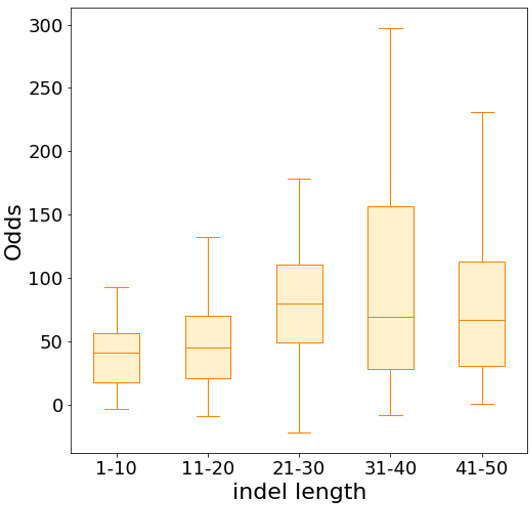
\includegraphics[width=0.6\columnwidth]{body/image/mid_new_odds.png}
\caption[no reads with variants from medium pile-up depth odds ratio]
{The vertical axis shows the EAGLE log odds ratio of variant to reference for indel variants, grouped by length (horizontal axis).  Plotted for variants occurring in regions with no reads from medium pile-up depth.}
\label{mid_new_odds}
\end{figure}


Finally, we look at the last row of Table~\ref{tab:mid-variants} we can see that our method still can help some variants that EAGLE cannot calculate because there is no pileup at the position. Figure~\ref{mid_new_odds} shows these variant odds calculated by EAGLE.

In this case, EAGLE can make more correct conclusions (that the position does contain variants) because we can find reads supporting the variants. It can be seen that compared to the previous case, regardless of the length of the indel, their Q3 is some distance higher, this result is also as we predicted (for example see Figure~\ref{mid_new_pileup}).


\begin{figure}[H]
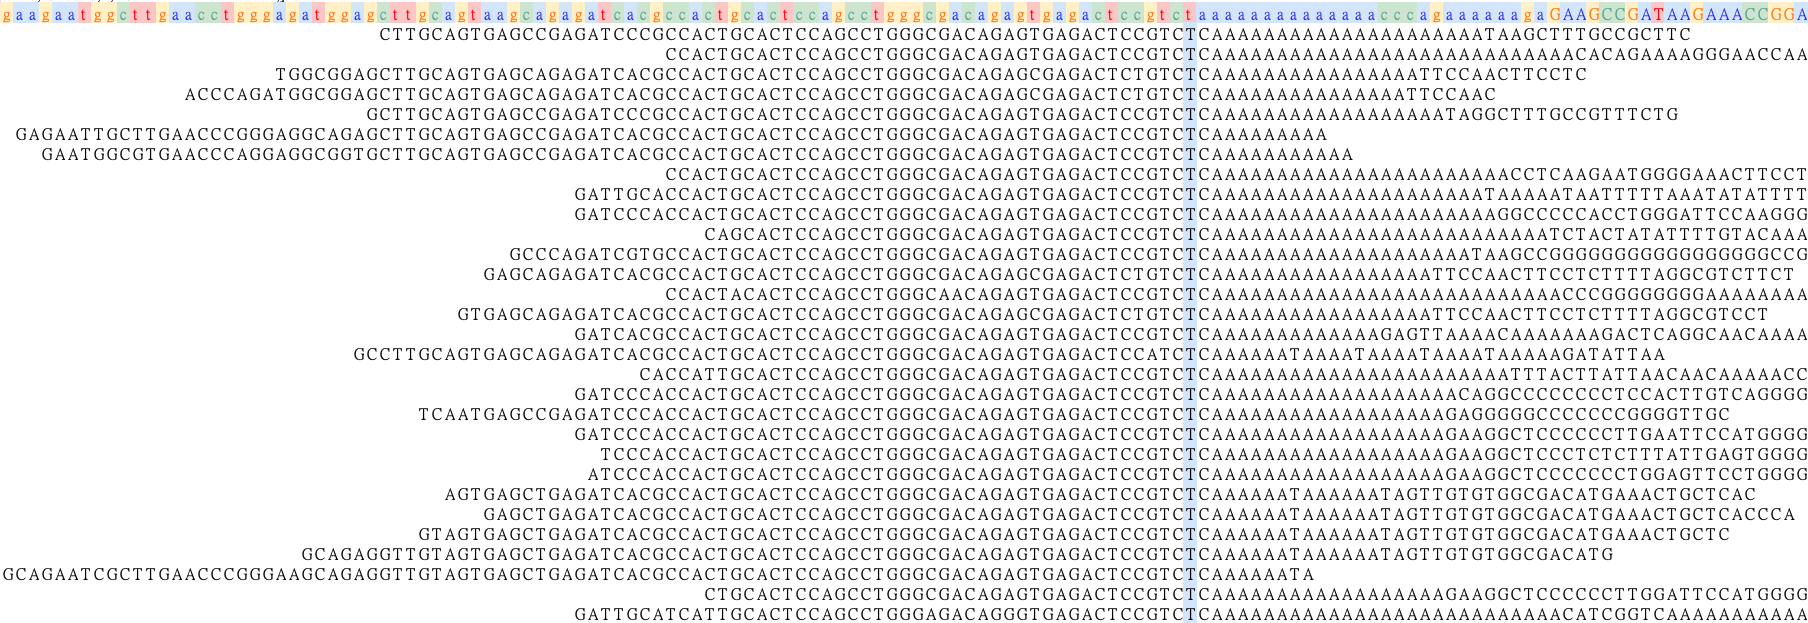
\includegraphics[width=1\columnwidth]{body/image/mid_new_pileup.png}
\caption[find new pileup reads in medium pile-up read depth]
{Reads found via the read-index are shown for a position for which standard read mapping to the doctored reference found no matching reads (an empty pile-up).
At top, the original reference genome sequence is shown.}
\label{mid_new_pileup}
\end{figure}

\section{Case 3: High pile-up read depth}
\begin{table}[ht]
    \centering
    \caption[High pile-up read depth variants]{High pile-up read depth variants}
    \vspace{-0.5cm}
    \begin{tabular}{|l|l|l|l|l|l|l|l|l|l|l|r|}
    \hline
    \textbf{Indel Length} & 
    \multicolumn{2}{c|}{\textbf{1--10}}  & \multicolumn{2}{c|}{\textbf{11--20}}  & \multicolumn{2}{c|}{\textbf{21--30}}  &
    \multicolumn{2}{c|}{\textbf{31--40}}  & \multicolumn{2}{c|}{\textbf{41--50}}   & 
    \textbf{Total}\\\hline
    \rowcolor{lightgray}
    \textbf{Unchanged}  & 
    44 & 25.9\%       &
    31 & 16.9\%     &
    36 & 19.6\%    &
    4 & 4\%     &
    0 & 0\%          &
    116\\ \hline
    \textbf{Changed} & 
    129 & 74.1\%       &
    152 & 83.1\%     & 
    148 & 80.4\%    & 
    96 & 96\%     &
    80 & 80\%        &
    605\\ \hline
    \rowcolor{lightgray}    
    \textbf{New}  & 
    \multicolumn{2}{c|}{26}      &
    \multicolumn{2}{c|}{17}     &
    \multicolumn{2}{c|}{16}      &
    \multicolumn{2}{c|}{100}    &
    \multicolumn{2}{c|}{120}       & 
    279\\ \hline
    \end{tabular}
    \label{tab:hi-variants}
\end{table}


Basically, in this case, we will observe results that are very similar to medium pile-up read depth, that's because there are quite a lot of reads, most positions can still produce pileup (Table \ref{tab:hi-variants}).

\begin{table}[H]
    \centering
    \caption[Changes in the number of variants with high pile-up read depth]{Changes in the number of variants with high pile-up read depth}
    \vspace{-0.5cm}
    \begin{tabular}{|l|c|c|c|c|c|r|}
    \hline
    \diagbox[dir=NW]{\textbf{$P[Alt]/P[REF] < 1$}}{\textbf{Indel length}} &
    \textbf{1--10} &     \textbf{11--20} &    \textbf{21--30} &    \textbf{31--40} &    \textbf{41--50} &    \textbf{Total}\\
    \hline
    \rowcolor{lightgray}
    \textbf{Before} &   6&     6&     2&    35&   36&    85 \\
    \hline
    \textbf{After} &   1&     0&     0&    1&   0&    2 \\
    \hline
    \end{tabular}
    \label{tab:hi-variants-change}
\end{table}

Interestingly, here we observe that the pile-up read depth rate is twice as high as that of the medium pile-up read depth, EAGLE initially judged that the position does not contain variation, but through our method we can complete more corrections than the medium pile-up read depth case. There are nearly 97\% of variants in Table \ref{tab:hi-variants-change} have been changed to the correct situation (Figures \ref{hi_new_REFread},\ref{hi_pileup_REFread} show some examples).

\begin{figure}[H]
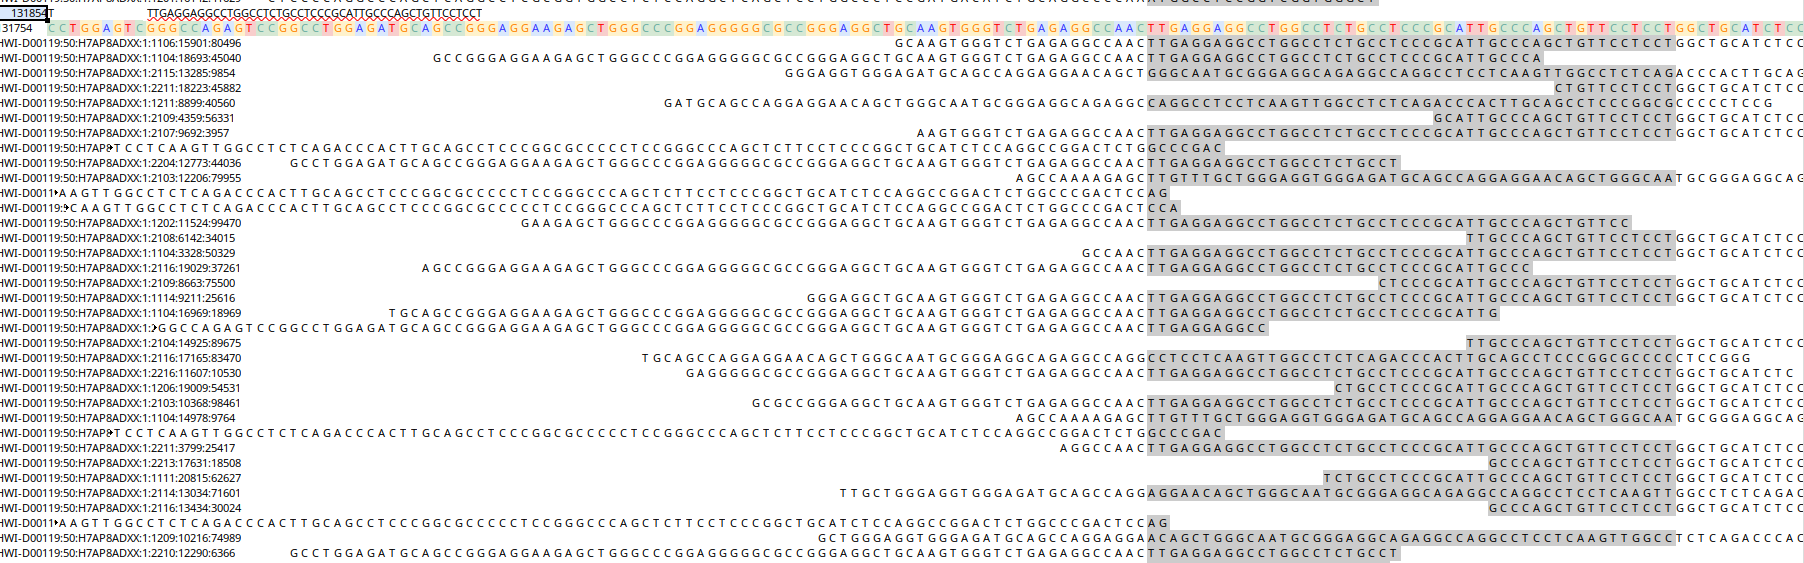
\includegraphics[width=1\columnwidth]{body/image/hi_new_REFread.png}
\caption[New reads in a region with high pile-up read depth]%
{Example of find large amount new reads supporting a variant in a region with high pile-up read depth.
\ExplainRedBracket.}
\label{hi_new_REFread}
\end{figure}

\begin{figure}[H]
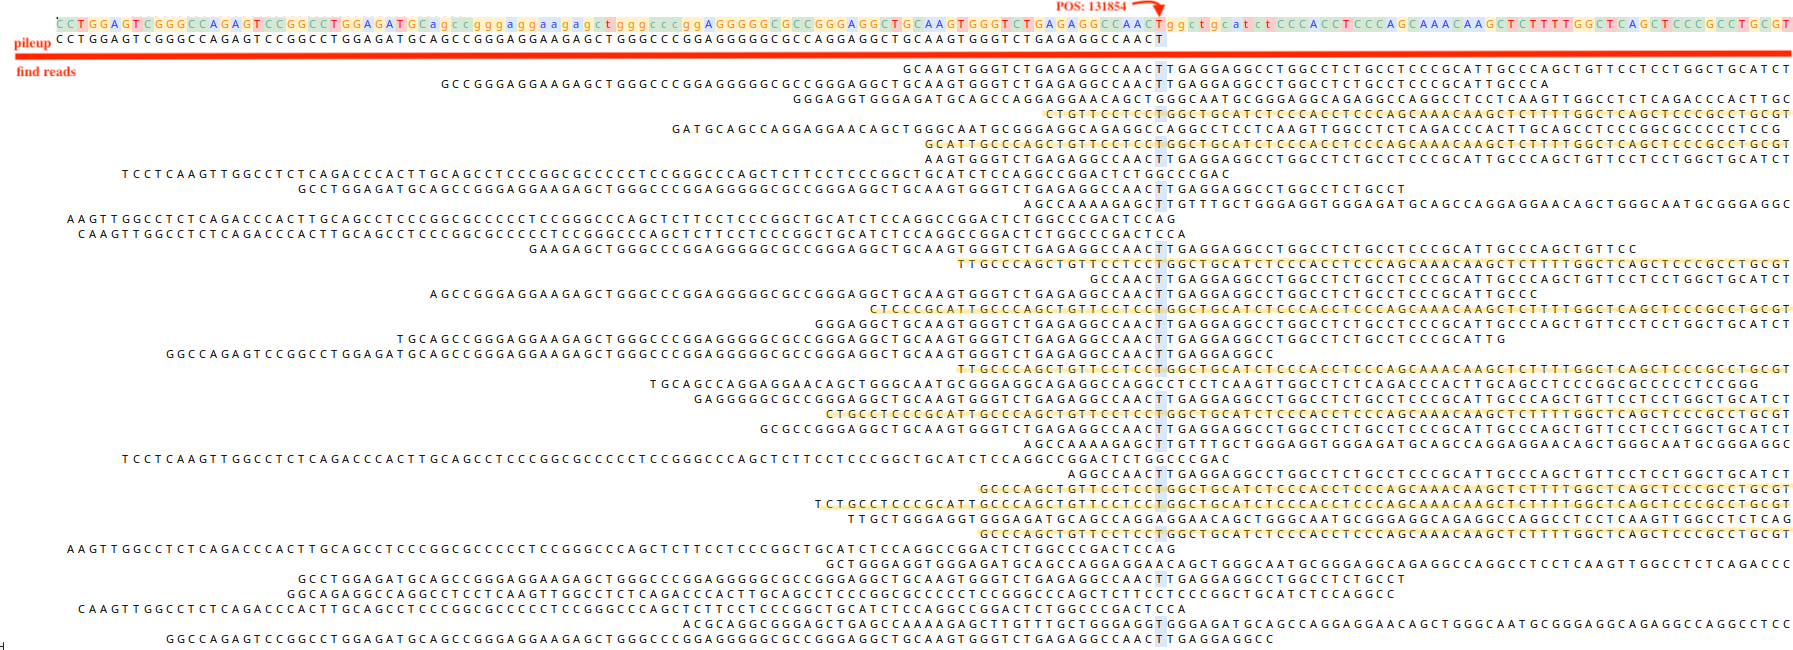
\includegraphics[width=1\columnwidth]{body/image/hi_pileup_REFread.png}
\caption[variant pileup in high pile-up read depth]
{Pileup after adding reads to high pile-up depth region.
At top, the doctored reference genome is shown with an arrow indicating where the simulated variant sequence was deleted from the original reference.}
\label{hi_pileup_REFread}
\end{figure}

Then, we look at the comparison of EAGLE odds in high pile-up read depth (Figure \ref{hi_odds_change}). It can be seen that compared with the previous example, it is very obvious that the longer the indel, the bigger the increase. However, we found many cases where the length of the mutation is greater than 50. This also shows that the more reads that we can find that would have been lost, the better we can reduce the impact of reference bias.

\begin{figure}[H]
\centering
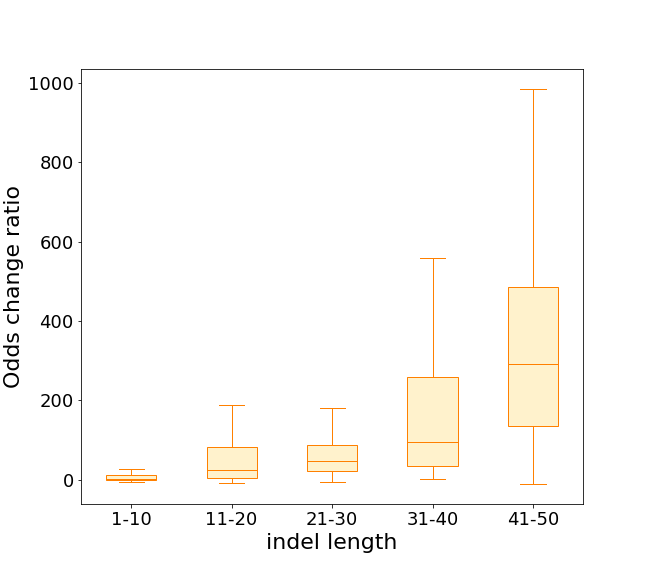
\includegraphics[width=0.6\columnwidth]{body/image/hi_odds_change.png}
\caption[high pile-up read depth odds change ratio]{The vertical axis shows the change in EAGLE log odds ratio of variant to reference for indel variants, grouped by length (horizontal axis).  Change here meaning the difference in the log odds ratio when when using the read index versus only using the pile-up.  Plotted for variants from high pile-up read depth regions.}
\label{hi_odds_change}
\end{figure}

Finally, we look at the last row of Table~\ref{tab:hi-variants}, we can see the same result as the previous case medium pile-up read depth. Figure~\ref{hi_odds_change} shows these variant odds calculated by EAGLE.

\begin{figure}[H]
\centering
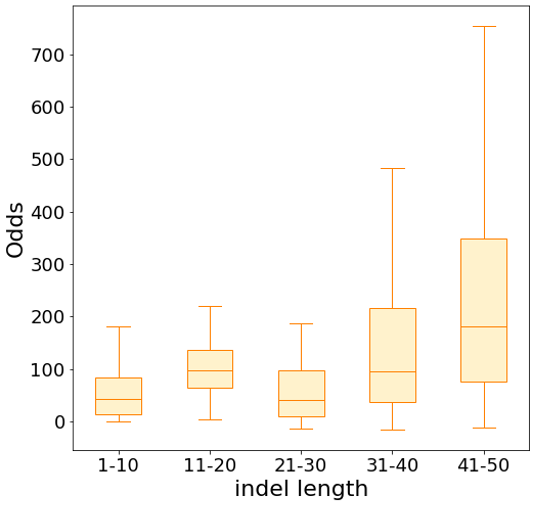
\includegraphics[width=0.6\columnwidth]{body/image/hi_new_odds.png}
\caption[no reads with variants from high pile-up depth odds ratio]{The vertical axis shows the EAGLE log odds ratio of variant to reference for indel variants, grouped by length (horizontal axis).  Plotted for variants occurring in regions with no reads from high pile-up depth.}
\label{hi_new_odds}
\end{figure}


\section{SNPs in dbSNP dataset}

There are 15,936,832 SNP variants form the dbSNP dataset, we random select 100,000 variants from the dataset, and the amount of matching pileup of the querying SNP variants are 50488. After joining our method, there are 22995 variants that have been changed as a result, we have looked at a few cases (Figure \ref{snp_new_ALTread},\ref{snp_pileup_ALTread},\ref{snp_new_REFread},\ref{snp_pileup_REFread}), we find many sequences that include the variants.


\begin{figure}[H]
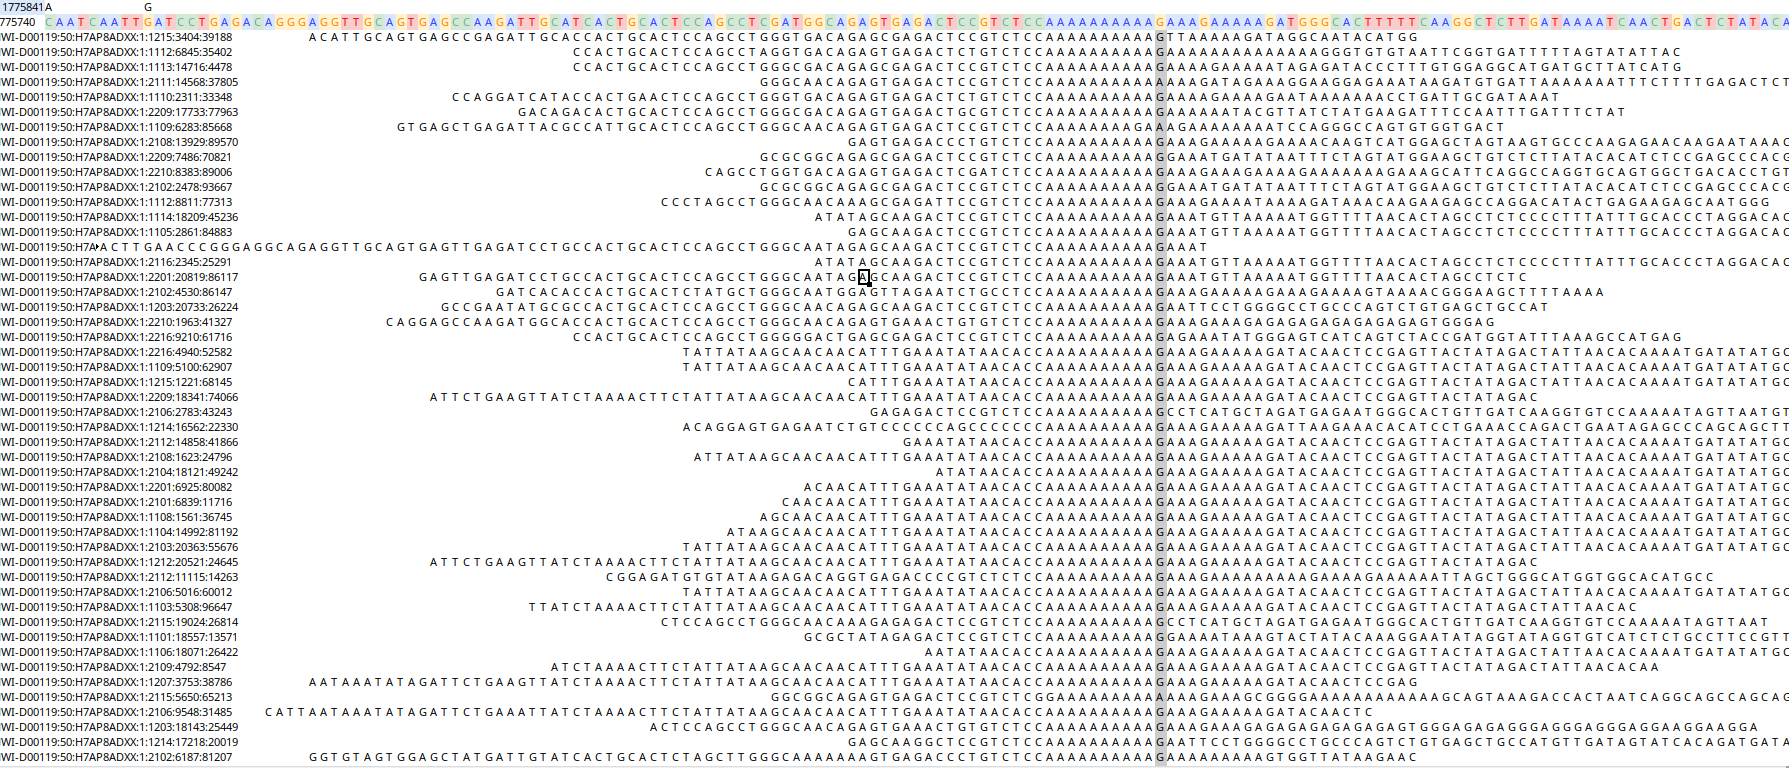
\includegraphics[width=1\columnwidth]{body/image/snp_new_ALTread.png}
\caption[SNP match reads]{Reads found via the read-index are shown for a SNP in dbSNP.}
\label{snp_new_ALTread}
\end{figure}

\begin{figure}[H]
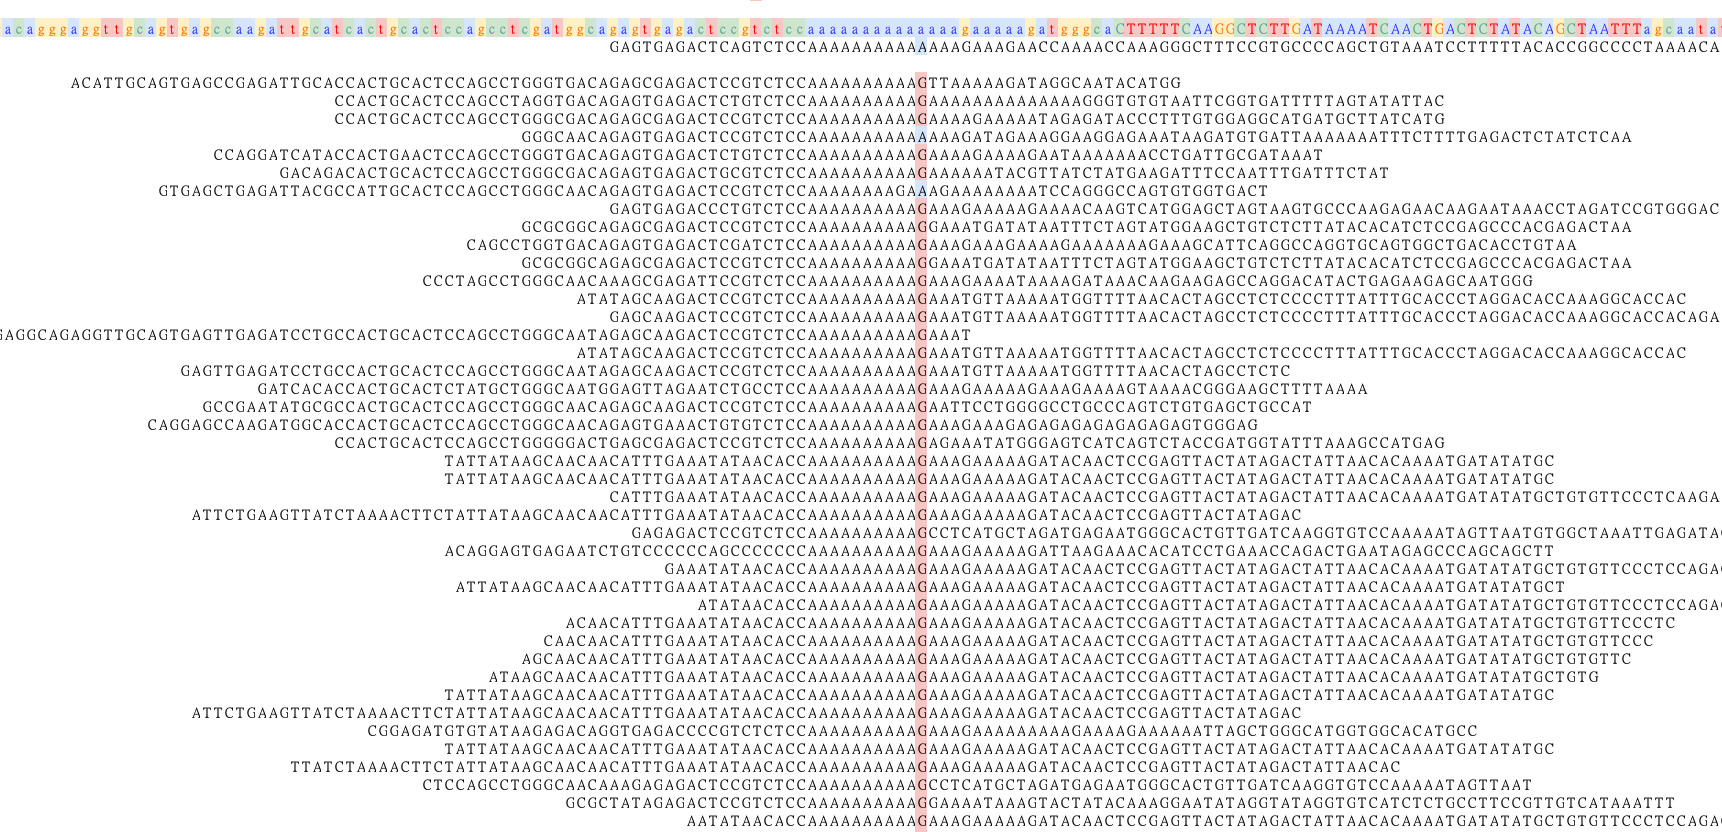
\includegraphics[width=1\columnwidth]{body/image/snp_pileup_ALTread.png}
\caption[Figure~\ref{snp_new_ALTread} pileup]{The pileup corresponding to the Figure~\ref{snp_new_ALTread} candidate variant.}
\label{snp_pileup_ALTread}
\end{figure}

\begin{figure}[H]
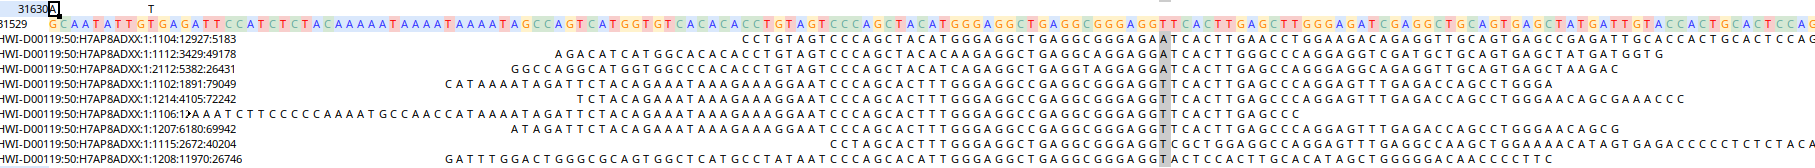
\includegraphics[width=1\columnwidth]{body/image/snp_new_REFread.png}
\caption[SNP worse match reads]{Reads found via the read-index are shown for a SNP in dbSNP.  In this particular case, those reads actually match the reference genome better.}
\label{snp_new_REFread}
\end{figure}

\begin{figure}[H]
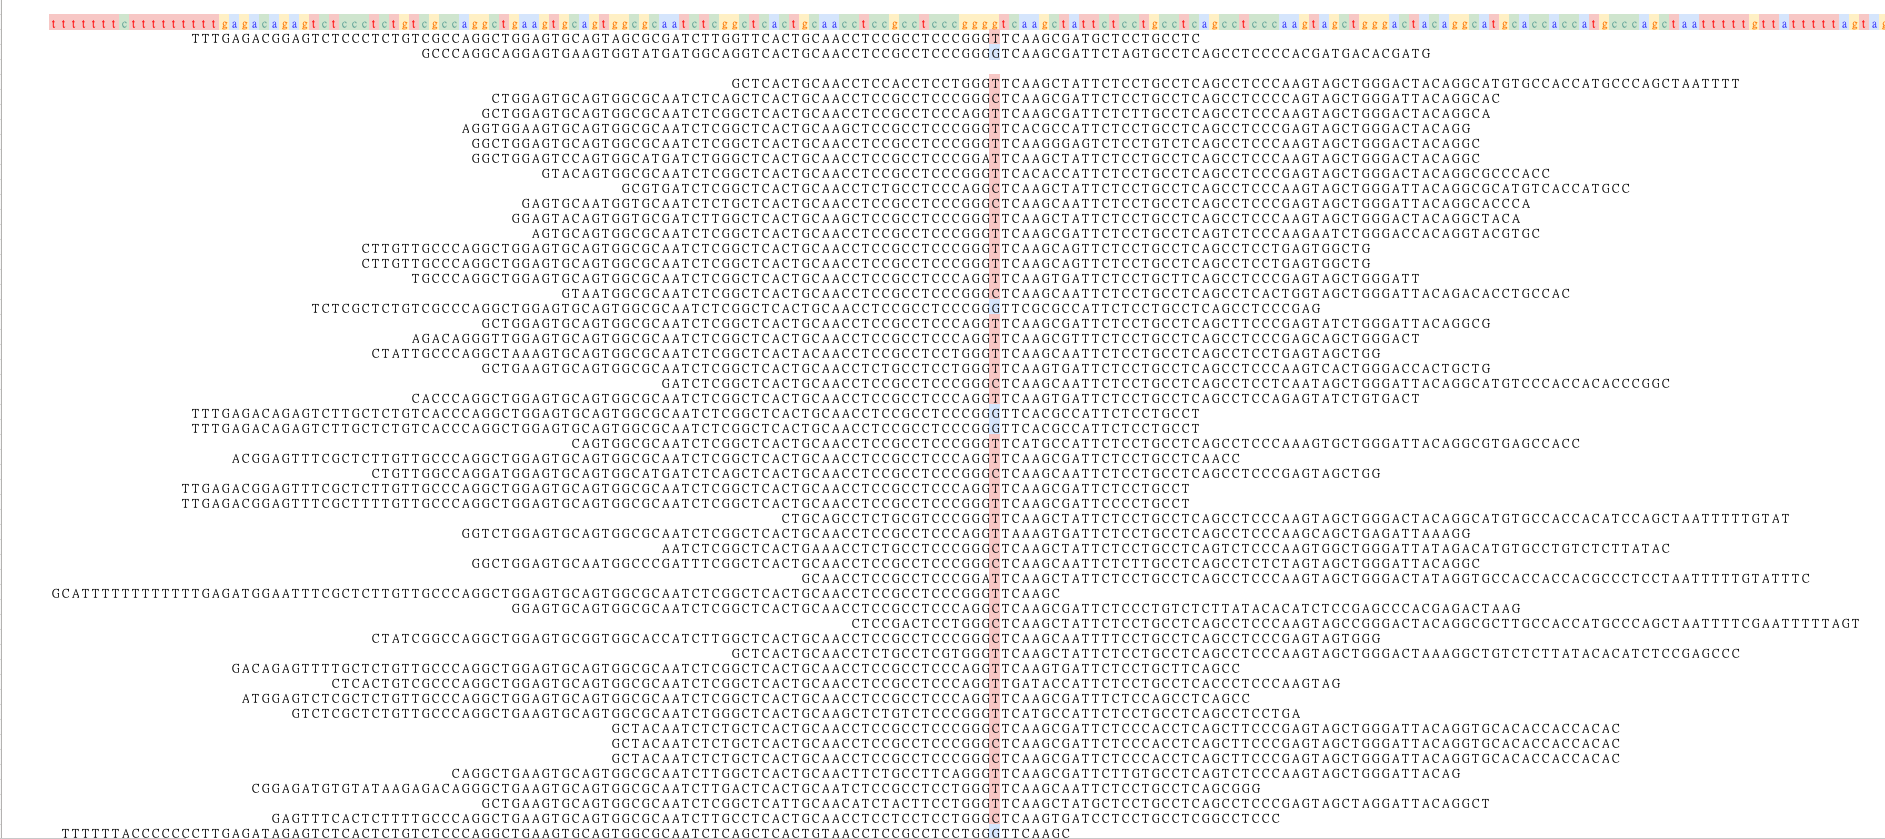
\includegraphics[width=1\columnwidth]{body/image/snp_pileup_REFread.png}
\caption[SNP worse match reads pileup]{The pileup corresponding to the Figure~\ref{snp_new_REFread} candidate variant.}
\label{snp_pileup_REFread}
\end{figure}

And we can find that the read we found gives EAGLE more basis for judgment, but the magnitude of the change is not very obvious in the SNPs (Figure \ref{snp_odds_change}), and most of them are less than 0. We speculate that the single-base nucleotide substitutions will not have a great impact on the alignment results.

\begin{figure}[H]
\centering
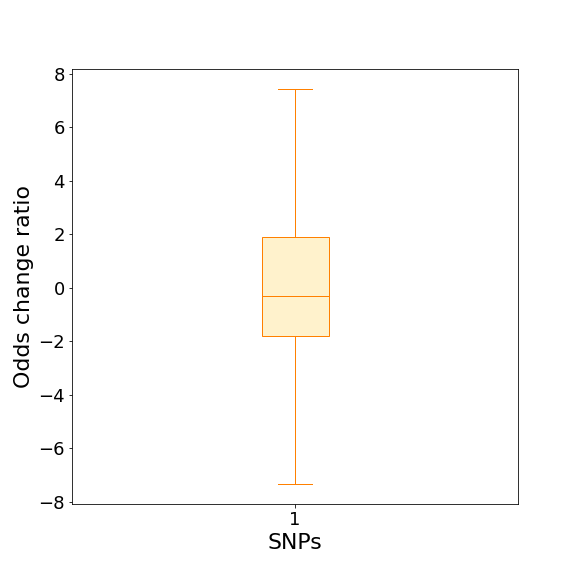
\includegraphics[width=0.6\columnwidth]{body/image/snp_odds_change.png}
\caption[SNPs odds change ratio]{SNPs odds change ratio.}
\label{snp_odds_change}
\end{figure}

\section{INDELs in dbSNP dataset}

There are 1,759,193 INDEL variants form the dbSNP dataset, we random select 10,000 variants from the dataset, and the amount of matching pileup of the querying INDEL variants are 5093. After using our new method, there are 2482 variants that have been changed as a result.  We have looked at a few cases (Figures~\ref{indel_new_ALTread},\ref{indel_pileup_ALTread},\ref{indel_new_REFread},\ref{indel_pileup_REFread}).

\begin{figure}[H]
\centering
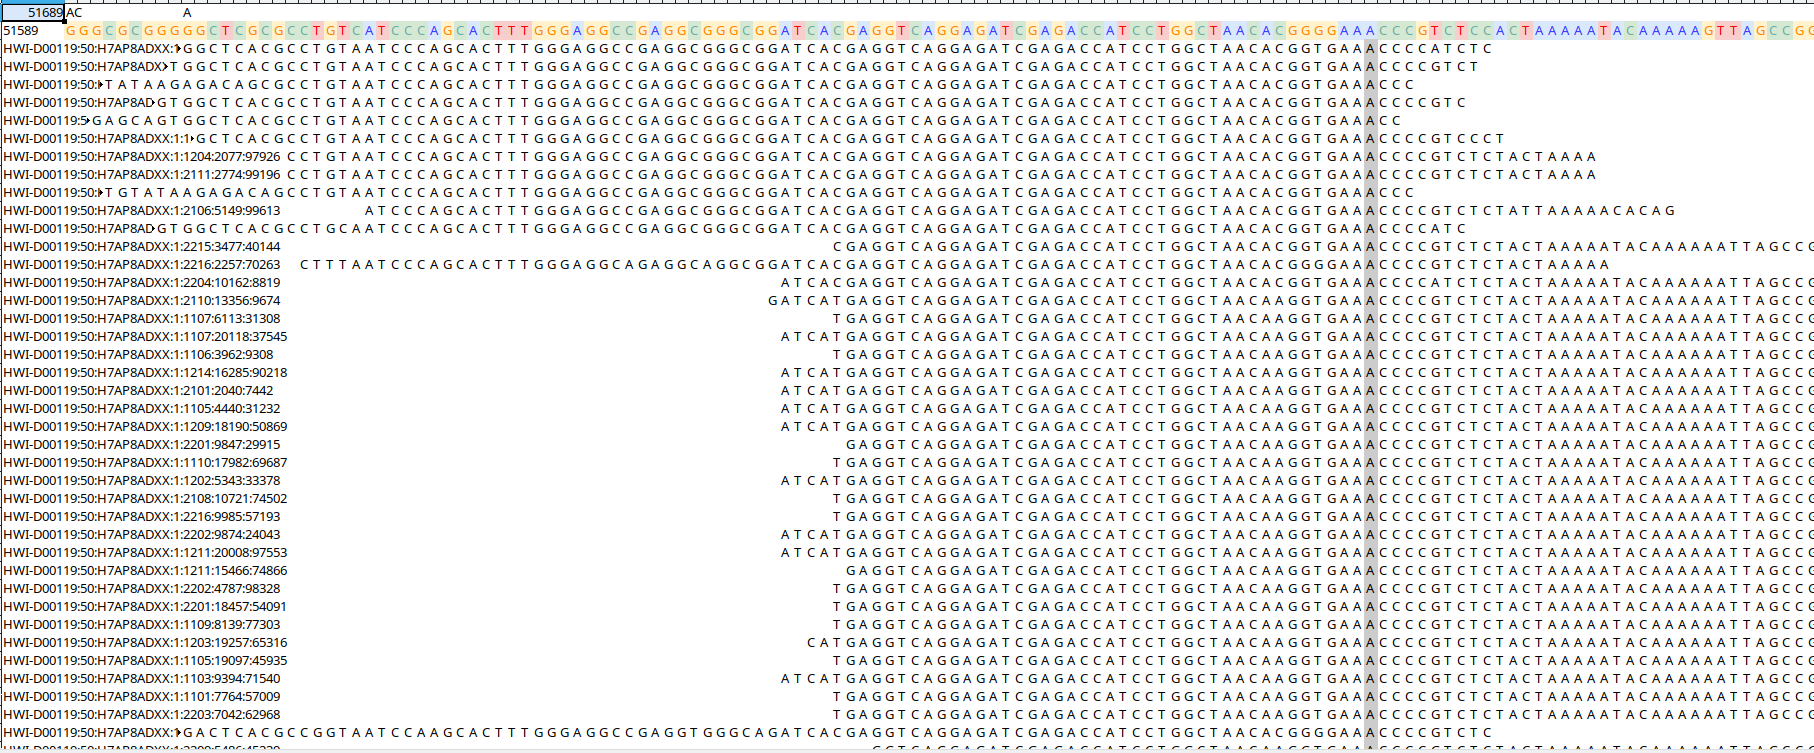
\includegraphics[width=1\columnwidth]{body/image/indel_new_ALTread.png}
\caption[INDEL match reads]{Matching reads with hypothetical sequence in INDEL}
\label{indel_new_ALTread}
\end{figure}

\begin{figure}[H]
\centering
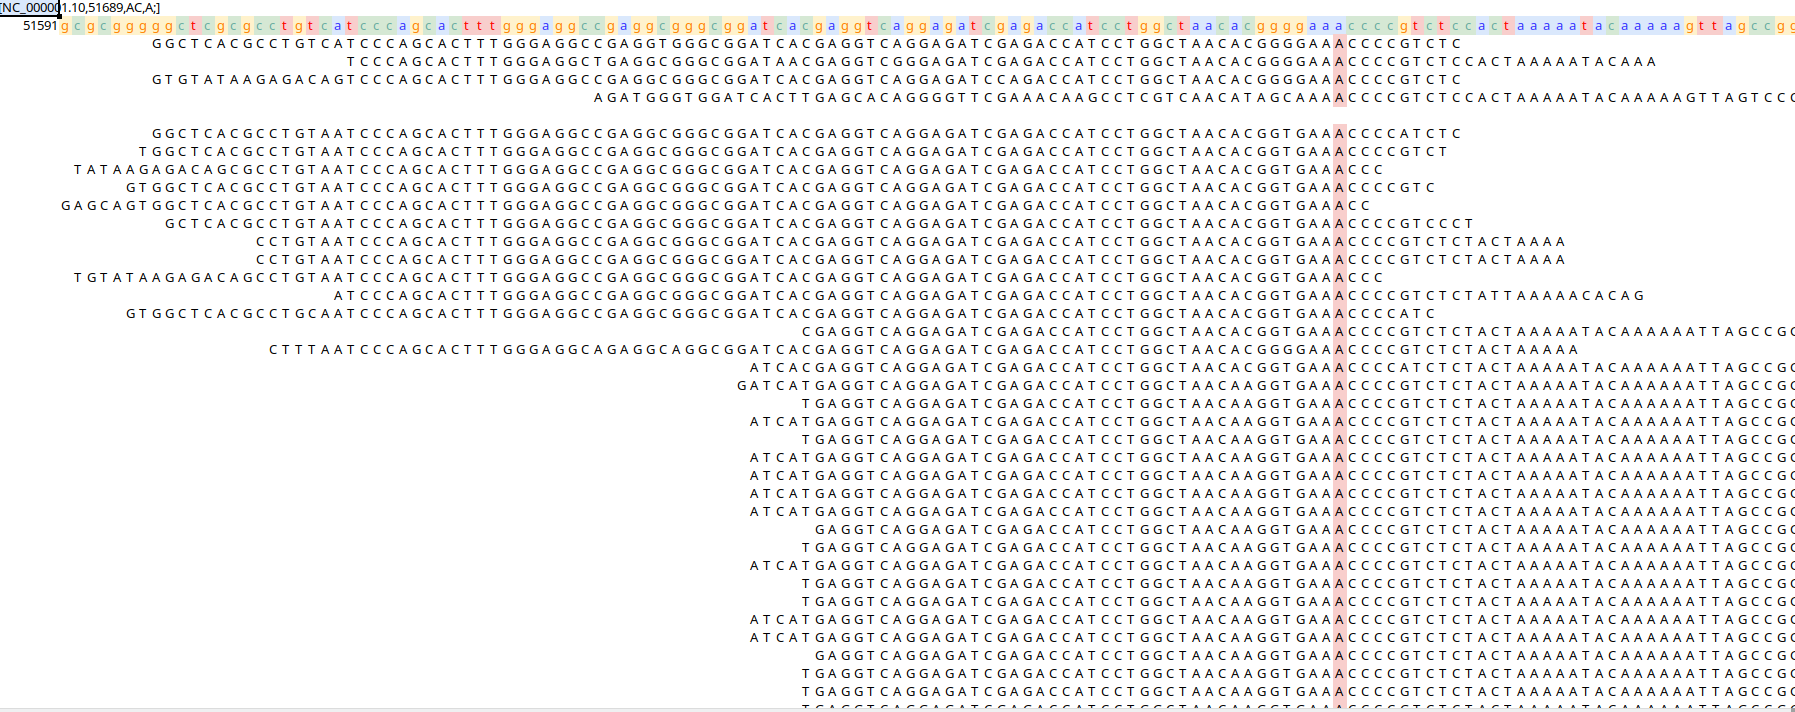
\includegraphics[width=1\columnwidth]{body/image/indel_pileup_ALTread.png}
\caption[Figure 4.22 pileup]{The pileup corresponding to the Figure \ref{indel_new_ALTread} variants.}
\label{indel_pileup_ALTread}
\end{figure}

\begin{figure}[H]
\centering
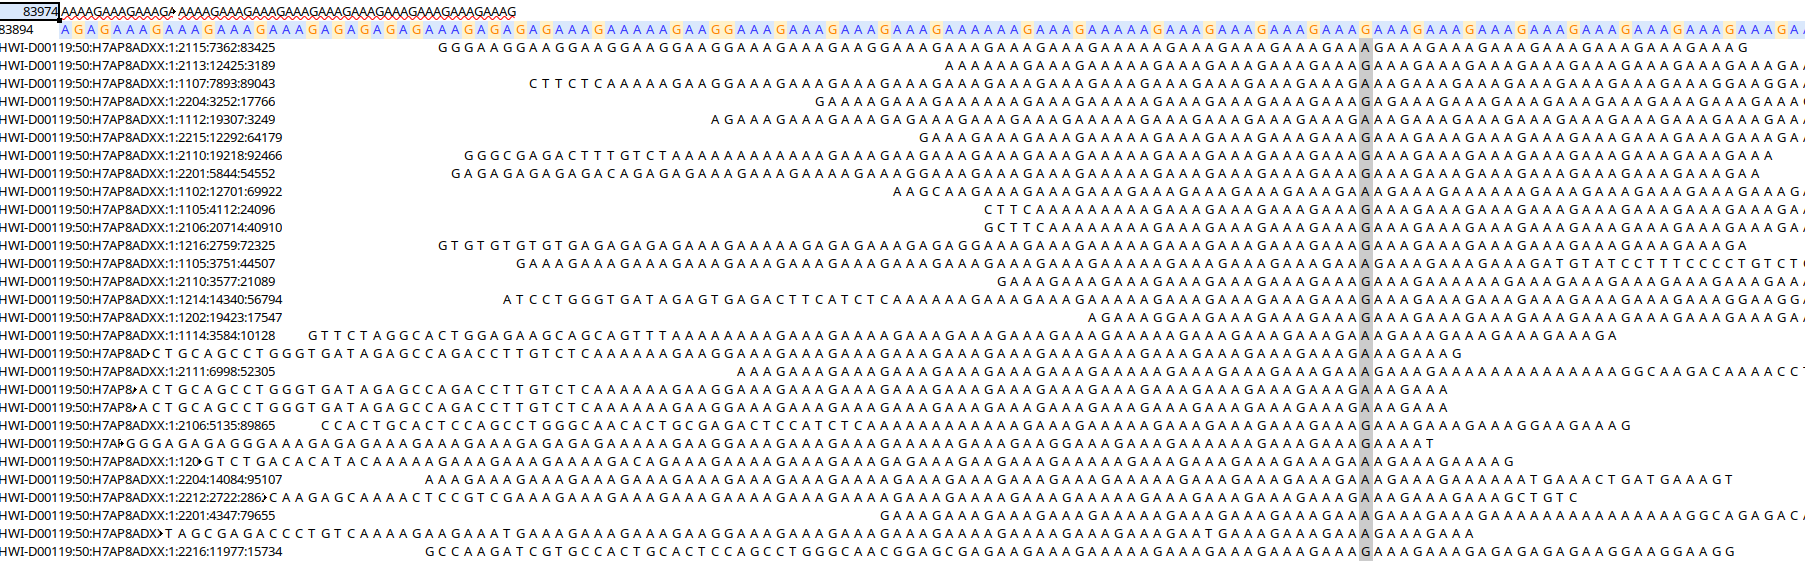
\includegraphics[width=1\columnwidth]{body/image/indel_new_REFread.png}
\caption[INDEL worse match reads]{Matching reads but more similar to reference sequence in INDEL.}
\label{indel_new_REFread}
\end{figure}

\begin{figure}[H]
\centering
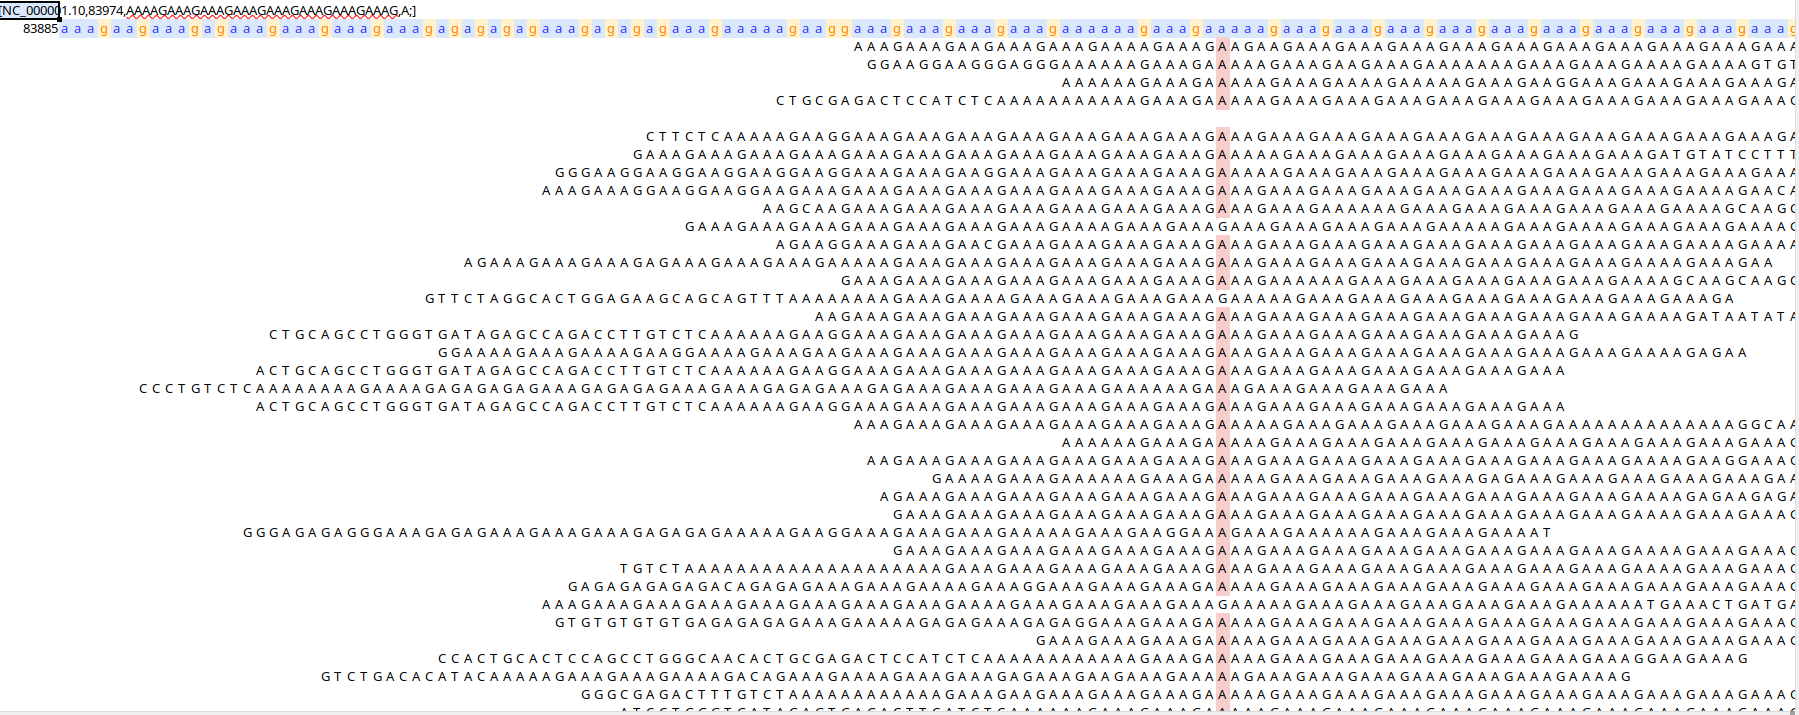
\includegraphics[width=1\columnwidth]{body/image/indel_pileup_REFread.png}
\caption[Figure 4.24 pileup]{The pileup corresponding to the Figure \ref{indel_new_REFread} variants.}
\label{indel_pileup_REFread}
\end{figure}

It can be seen that the reads we found gave EAGLE more evidence for judgment, and that the magnitude of change in INDEL was significantly greater than SNP, just like the experiment we simulated before.

\begin{figure}[H]
\centering
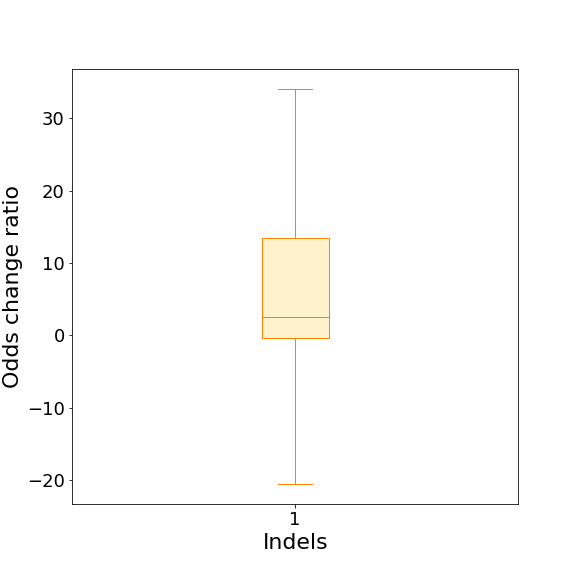
\includegraphics[width=0.6\columnwidth]{body/image/indel_odds_change.png}
\caption[INDEL odds change ratio]{INDEL odds change ratio.}
\label{indel_odds_change}
\end{figure}

\section{Execution time and memory consumption}

Finally, let’s discuss our execution time and memory consumption, our test data are as follows Table~\ref{tab:dataset}, test environment as Figure~\ref{environment}.

\begin{table}[ht]
    \centering
    \caption[Test Dataset]{Test Dataset}
    \vspace{-0.5cm}
    \resizebox{\textwidth}{25mm}{
    \begin{tabular}{|l|l|l|l|}
    \hline
     &
    \textbf{Reference Genome} &    \textbf{Read} &   \textbf{VCF} \\
    \hline
    \rowcolor{lightgray}
    \textbf{Dataset} &  
    
    \begin{tabular}{p{6cm}}
     Genome Reference Consortium Human Build 37 patch release 13 version
    \end{tabular}
    
    &\begin{tabular}{p{6cm}}
     Garvan NA12878 HG001 HiSeq Exome
    \end{tabular} &
    \begin{tabular}{p{6cm}}
     Single Nucleotide Polymorphism Database (dbSNP)
    \end{tabular} \\
    \hline
    \textbf{File Size} &   3.1G &    5G &  669.7MB \\
    \hline
    \end{tabular}}
    \label{tab:dataset}
\end{table}
\vspace{0.5cm}
\begin{figure}[H]
    \centering
    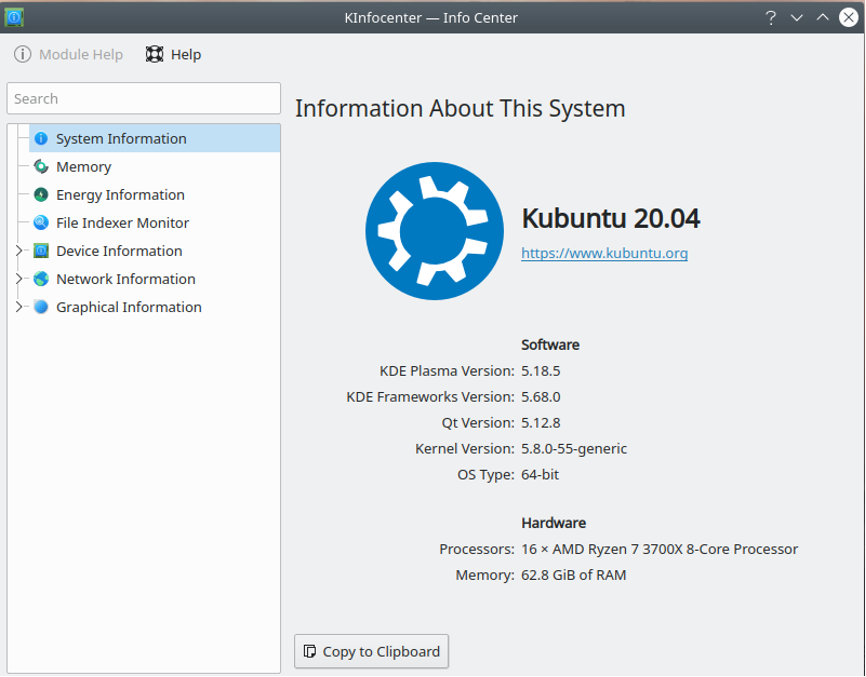
\includegraphics[width=0.8\columnwidth]{body/image/environment.png}
    \captionsetup{labelfont=bf}
    \renewcommand{\baselinestretch}{1.0}
    \caption[Test Environment]{Test Environment.}
    \label{environment}
\end{figure}

Experimenting with the above conditions, first we can see that the memory we consume is 11.64G, and the memory consumed by EAGLE is 0.36G, we can find that the memory space we need is indeed much larger than the original EAGLE. This is because we need to access read-index, reference-index and read files to complete quick searches, so the memory size we need is closely related to these three.
But what we care most about is our execution speed. The time taken by EAGLE is 3618.18 seconds and our method is 6426.28 seconds. Although it seems to take a lot of time, we can find out that we have increased by carefully analyzing our execution time. A large part of the time is to index the read. The time it takes is 1649.33 seconds, but the time to search is very quick, as shown in Figure \ref{search_time}, and a part of the time is because we find more reads, the calculation added by EAGLE Time. Considering this situation, we can say that the added time is relatively small.

\begin{figure}[H]
\centering
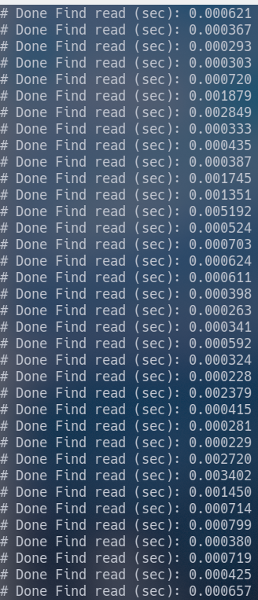
\includegraphics[width=0.4\columnwidth]{body/image/search_time.png}
\caption[searching time]{searching per hypothetical sequence time.}
\label{search_time}
\end{figure}
